\documentclass[border=2mm]{standalone}
\usepackage{pgfplots}
\usepgfplotslibrary{colormaps}
\pgfplotsset{
	compat=1.13,
	% either load the colormap here ...
	%        colormap/gray,
}
\begin{document}
	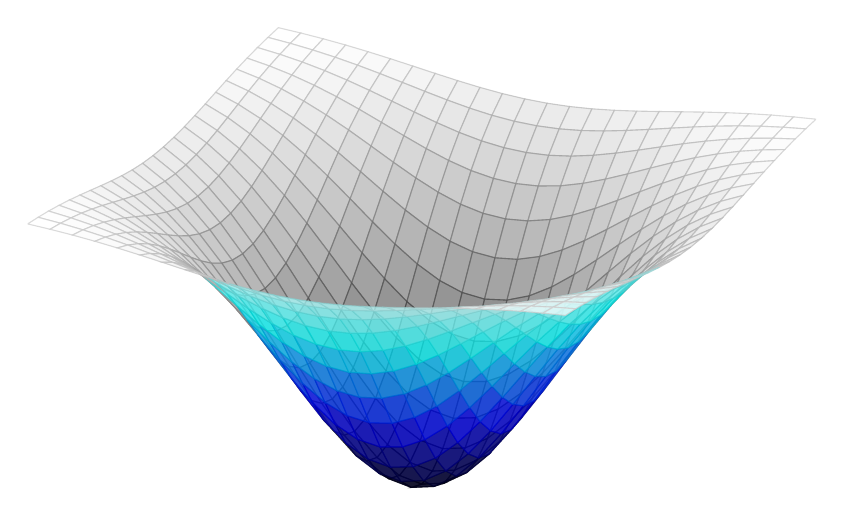
\begin{tikzpicture}
		\begin{axis}[
			height=10cm,
			hide axis,
			xlabel=$x$,
			ylabel=$y$,
			% ... or here
			colormap/gray,
			]
			\addplot3[
			domain=-1.5:1.5,
			opacity=0.7,
			surf,colormap/cold,
			%mesh/interior colormap name=hot, %works
			mesh/interior colormap name=gray, %doesn't work
			] {-exp(-x^2-y^2)};
		\end{axis}
	\end{tikzpicture}
\end{document}